\documentclass[12pt, twoside,a4paper]{article}
\oddsidemargin = 10pt
\textwidth = 430pt

\usepackage{fullpage}	 %to make smaller margins
\usepackage{graphicx}
%\usepackage[utf8]{inputenc}
%\usepackage[T1]{fontenc}
%\usepackage{url}

\usepackage[hidelinks]{hyperref}
\usepackage{pdfpages}
\usepackage{placeins}
\usepackage{graphicx}
\usepackage[font=small,labelfont=bf]{caption}
\usepackage{subfig}

%\usepackage{subcaption}
\usepackage{enumerate}
\usepackage{amsmath}
\usepackage{listings} %for showing program code
\usepackage{bm}
\usepackage{wrapfig}
\usepackage{lipsum}
\usepackage{float}
\usepackage{titlesec}	
\usepackage{amsfonts}
\usepackage{amssymb}
\usepackage[comma,authoryear]{natbib}
\usepackage{epstopdf}
\usepackage{array}
\usepackage{blindtext}
\usepackage{tabularx}
\usepackage{glslListings} 

\newcommand{\vomega}{\vec{\omega}}
\newcommand{\x}{\mathbf{x}}
\newcommand{\cs}{C_{\phi}(\eta)}
\newcommand{\csinv}{C_{\phi}(1/\eta)}
\newcommand{\ce}{C_{\mathbf{E}}(\eta)}
\newcommand{\gl}[1]{\texttt{\nolinkurl{#1}}}
%\titlespacing*{\chapter}{0pt}{-10pt}{20pt}
%\titleformat{\chapter}[display]{\normalfont\huge\bfseries}{}{35pt}{}

%\setlength{\intextsep}{0pt} %to make wrapfigures beautiful
%\setlength{\oddsidemargin}{0.5cm}
%\setlength{\evensidemargin}{-0.5cm}
\begin{document}
\section{Errata}
\subsection{Chapter 3 - Theory}
\begin{description}
	\item [Page 15, paragraph 1]: \emph{visible light} must be replaced with \emph{visible electromagnetic radiation}. The last sentence (``Instead explicitly noted, [...]'') can be removed. 
	\item [Page 15, paragraph 1]: The wavelengths of infrared and ultraviolet are swapped. It should be ``between the 380nm of the ultraviolet and the 750nm of the infrared''.
	\item [Page 16, paragraph 1]: The terms in photometry are \emph{luminous energy} and \emph{luminous flux}, instead of \emph{radiant energy} and \emph{radiant flux}.
	\item [Page 17, caption 3.2]: It is the opposite in fact. By shrinking the area, we retain more or less the same irradiance, while the measured flux is different. So, the caption should read: \emph{Irradiance versus power. For the two surfaces $A$ and $B$, the received irradiance $E$ is the same, while the two measured fluxes $\Phi_A$ and $\Phi_B$ are different, as the area of $B$ is twice as the one of $A$.}
	\item [Page 20, table 3.2]: Some quantities in the table are not correct. The radiance quantities require both a different delta function in order to work. We must then distinguish between flux in a point and \emph{total} flux emitted by the source. In the directional case, the flux is zero (as they have no source) and the total flux is infinite (as a directional light is infinitely large). In the point case, we have a total flux of four times $\pi$ the intensity, that is all concentrated in the origin. 

\renewcommand{\arraystretch}{1.8}
\begin{table}[!ht]
    \centering
    \begin{tabularx}{0.95\textwidth}{|X|X|X|}
    \hline
    Quantity   & Directional light & Point light \\ \hline
    Cosine term       & $\cos\theta = \vec{n} \cdot \vomega_l$ & $\cos\theta = \frac{(\x - \x_l) \cdot \vec{n}}{|\x - \x_l|}$     \\ \hline
    $\Phi(\x)$ Flux       & $0$                  & $4 \pi I\ \delta(\x_l - \x)$           \\ \hline
    $\Phi$ Total Flux       & $\infty$                  & $4 \pi I $           \\ \hline
		$E(\x)$ Irradiance & $L \cos\theta $                 & $I \frac{\cos\theta}{|\x_l - \x|^2}$          \\ \hline
    $I(\x,\vomega)$ Intensity  & 0                 & $I\ \delta(\x_l - \x)$           \\ \hline
    $L(\x,\vomega)$ Radiance   & $L\; \delta(\vomega - \vomega_l)$               & $\frac{I}{|\x_l - \x|^2} \ \delta(\vomega - \frac{(\x - \x_l)}{|\x - \x_l|})$           \\ \hline
    \end{tabularx}
\caption{Different radiometric values for simple light sources.}
\label{table:radio}
\end{table}
 \item [Page 20, 21 and 27]: The $L_o$ and $\vomega_o$ terms should be replaced by $L_r$ and $\vomega_r$ (reflected radiance), as the former two are reserved for the rendering equation formulation.
\item [Page 20, paragraph 2]: \emph{The BRDF states that the incoming [...]} shold be replaced with \emph{The BRDF states that the incoming irradiance and the outgoing radiance are proportional.}
\item [Page 20, paragraph 1]: The properties listed are generally attributed to \emph{physically based} BRDF functions.
\item [Page 23, bottom]: the $\vec{h}$ vector should be defined with the reflection vector:
$$
\vec{h} = \frac{\vomega_r + \vomega_i}{\left\| \vomega_r + \vomega_i \right\|}
$$
\item [Page 25, paragraph 2]: The equation misses a subscript in the emissing term. Moreover, the visibility term is already included into the incoming radiance $L_i$. So the right equation is:
$$
L_o(\x, \vomega_o) = L_e(\x, \vomega_o) + \int_{2\pi} f(\x, \vomega_i, \vomega_o) L_i(\x, \vomega_i) (\vec{n} \cdot \vomega_i) d\vomega_i
$$
And the same correction must be done in the renderign equation at page 28:
$$
L_o(\x_o,\vomega_o) = L_e(\x_o,\vomega_o) + \int_A \int_{2\pi} S(\x_i, \vomega_i, \x_o, \vomega_o) L_i(\x_i,\vomega_i) (\vec{n} \cdot \vomega_i) d\vomega_i d A_i
$$
\item [Page 28, paragraph 5]: the directional derivative equation is not spectral, and should be changed as
$$
(\vec{\nabla} \cdot \vomega) L(\x, \vomega) = \frac{\partial L}{\partial x} \vomega_x + \frac{\partial L}{\partial y} \vomega_y + \frac{\partial L}{\partial z} \vomega_z
$$
\item [Page 32, paragraph 1]:  $1/\sigma_t$ is the \emph{mean free path}, while the converse of the reduced extinction coefficient, $1/\sigma_t'$, is called the \emph{transport mean free path}.
\item [Page 32, and throughout the thesis]: what we call \emph{transmission coefficient} is commonly referred as \emph{effective transport coefficient} in literature.
\item [Page 37, equation 3.15]: it should be corrected as
$$
\ce = \frac{3}{4\pi} \left(\frac{2\pi}{3} - \int_{2\pi} R(\eta,\vomega) (\vec{n}_o \cdot \vomega)^2 d \vomega \right) = \frac{1}{2}(1 - 3 C_2) \\
$$
with a changed cosine squared term in the integral.
\end{description}
\subsection{Chapter 5 - Implementation}
\begin{description}
\item [Page 80]: The code for the LCG noise is wrong. It should be replaced with the following.
\begin{lstlisting}[language=GLSL,label=lst:sinegenerator]
highp float noise_lcg(vec2 co, int size)
{
  uint k = co.x + size * co.y;
  uint b = 3125;
  uint c = 49;
  uint result = 1; /* have to start somewhere */

  for (;k > 0;k>>=1)
  {
    if ((k & 1) == 1) result = result * b + c;
    c += b * c;
    b *= b;
  }
  return float(result) / 4294967296.0f;
}
\end{lstlisting}
Despite giving a comparable result now (see Figure \ref{fig:noise}), it is still a less viable solution that the LSR noise, as we need to generate only one random number per pixel.
\begin{figure}
\centering
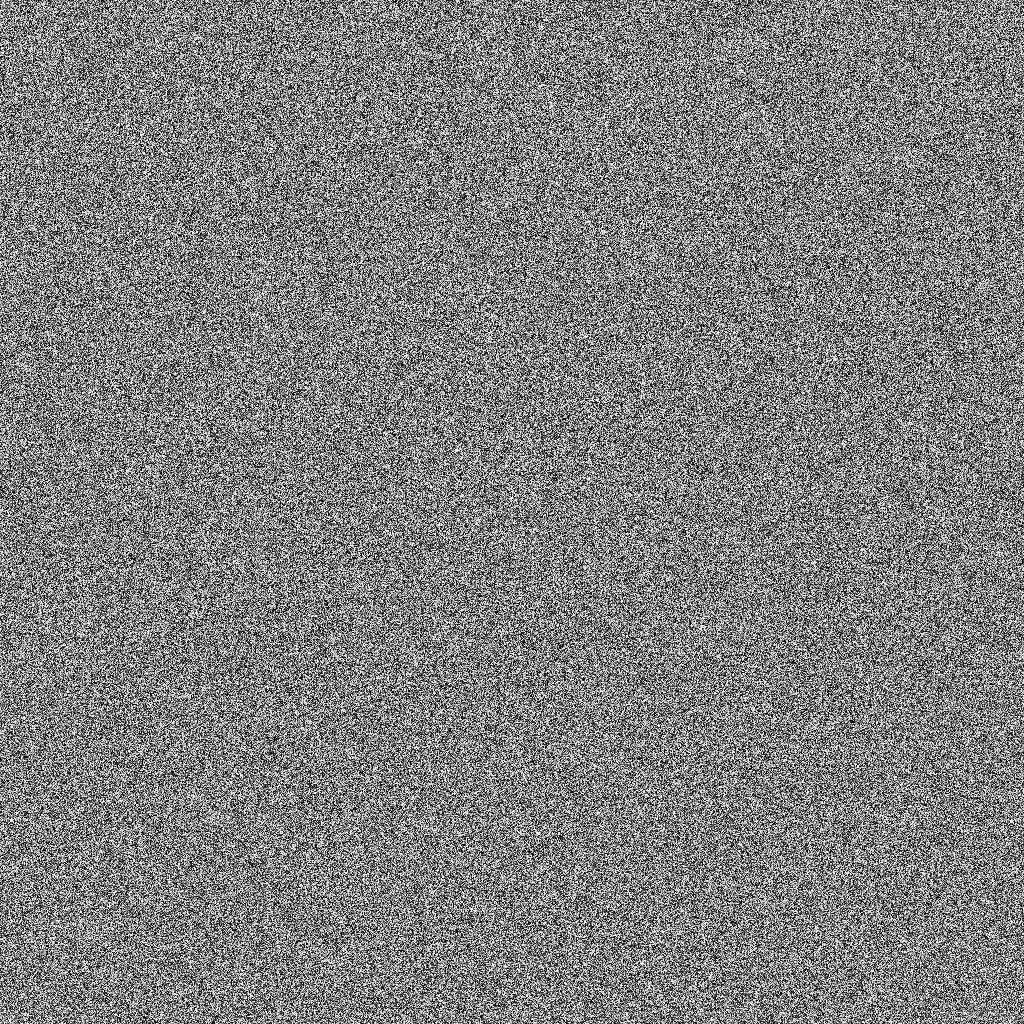
\includegraphics[width=0.6\linewidth]{n.png}
\caption{Corrected LCG noise.}
\label{fig:noise}
\end{figure}
\item [Page 88]: the distance $\|\x_l - \x_i\|$ must be squared in order to get the right radiance term in point lights. While listing 5.13 is correct, two equations in this page are not: 
\begin{equation*}
R^{t,k}(\x_o) = {I_l} \sum_{i = 1}^N  \frac{S(\x^{t,k}_i, \frac{\x_l - \x_i}{\|\x_l - \x_i\|}, \x_o, \vomega_o)}{{\|\x_l - \x_i\|^2}} \exp\left(\sigma_{tr} r^{t,k}_i\right), \ \ t \in [0,T], \ \ k \in [0,K-1] 
\end{equation*}
\begin{equation*}
L(\x_i, \vomega_l(\x_i)) = \begin{cases}
L_l & \text{if l is directional with $\vomega_l$, $L_l$} \\
 \frac{I_l}{\|\x_l - \x_i\|^2} & \text{if $l$ is point with $\x_l$, $I_l$}
\end{cases} \\
\end{equation*}
\end{description}
\subsection{References}
\begin{description}
\item {[Torrance and Sparrow 1992]} is {[Torrance and Sparrow 1967]}, as the original submission was in JOSA (DOI: \url{http://dx.doi.org/10.1364/JOSA.57.001105}).
\item {[Born and Emil 1999]} is {[Born and Wolf 1999]}.
\end{description}

\end{document}
